\documentclass[aspectratio=169,11pt]{beamer}
\usepackage[T1]{fontenc}
\usepackage[utf8]{inputenc}
\usepackage[french]{babel}
\usepackage{lmodern}
\usepackage{booktabs}
\usepackage{tabularx}
\usepackage{tikz}
\usetikzlibrary{positioning,arrows.meta,calc,fit}

\usetheme[progressbar=frametitle,numbering=fraction]{metropolis}

\definecolor{nuit}{HTML}{14213D}
\definecolor{papier}{HTML}{F7F6F2}
\definecolor{bleu}{HTML}{1F5FAD}
\definecolor{bleuclair}{HTML}{DCE7F6}
\definecolor{orange}{HTML}{C2581F}
\definecolor{orangeclair}{HTML}{F6E6DA}
\definecolor{vert}{HTML}{2E7D32}
\definecolor{gris}{HTML}{4A5568}
\definecolor{trait}{HTML}{DDD8CC}

\setbeamercolor{normal text}{fg=nuit,bg=papier}
\setbeamercolor{frametitle}{fg=papier,bg=nuit}
\setbeamercolor{progress bar}{fg=bleu,bg=bleuclair}
\setbeamercolor{alerted text}{fg=orange}
\setbeamercolor{title separator}{fg=bleu}
\setbeamercolor{background canvas}{bg=papier}

\tikzset{
  carte/.style={draw=trait,fill=white,rounded corners=4pt,align=center,inner sep=6pt,font=\small,execute at begin node={\hyphenpenalty=10000}},
  fleche/.style={-{Stealth[length=2.5mm]},thick,bleu},
}

\title{Dessiner un graphe directement en espace écran}
\subtitle{Jalon 2 : l'espace écran change-t-il le dessin ? (partie de Yani)}
\author{Melissa Colin \and Quentin Lopez \and Yani Haouchine}
\institute{ENSEIRB-MATMECA 3A, projet semestriel \quad·\quad Encadrant : Romain Giot (LaBRI)}
\date{18 décembre 2026}

\begin{document}

\maketitle

\begin{frame}{La question du sujet, sur un exemple}
\centering
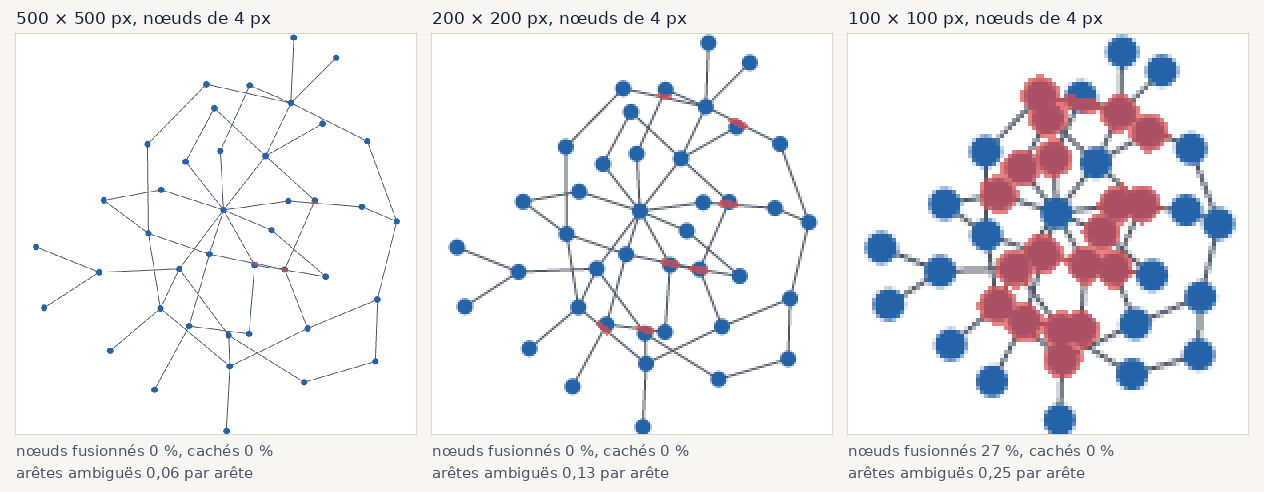
\includegraphics[width=0.93\textwidth]{tailles.png}

\vspace{0.1cm}
\small Le \textbf{même} dessin de Kamada-Kawai à trois tailles d'écran, nœuds de 4 px ; en rouge, les défauts de l'image rendue.\\[2pt]
\footnotesize\textcolor{gris}{Stress et mesures de la littérature identiques sur les trois : elles ignorent la taille d'affichage.}
\end{frame}

\begin{frame}{Mesurer l'image rendue, pas la géométrie}
\small Calculées sur la couverture exacte de chaque nœud et de chaque arête, pixel par pixel (notre rasteriseur), à la taille d'affichage.

\vspace{0.3cm}
\centering
\footnotesize
\begin{tabularx}{\textwidth}{@{}l X@{}}
\toprule
\textbf{Mesure} & \textbf{Définition} \\
\midrule
Nœuds cachés & part des nœuds visibles à moins de 50 \% (recouverts par d'autres, ou hors du cadre) \\
Nœuds fusionnés & nœuds collés à un autre une fois pixelisés : $N - $ nombre de taches d'encre \\
Arêtes ambiguës & paires (arête, nœud qu'elle ne relie pas) qui partagent un pixel \\
Arêtes confondues & part de l'encre des arêtes couverte par deux arêtes ou plus \\
\bottomrule
\end{tabularx}

\vspace{0.3cm}
\begin{tikzpicture}
  \node[carte,draw=orange,fill=orangeclair,text width=0.9\textwidth,align=left,inner sep=4pt] {\small Deux disques à 0,3 px l'un de l'autre ne se recouvrent pas : aucune mesure géométrique ne le voit. Une fois pixelisés, ils forment une seule tache.};
\end{tikzpicture}

\vspace{0.1cm}
\scriptsize\textcolor{gris}{24 tests à réponse connue (aire de la lentille, fusion sans recouvrement, invariance par translation\ldots). 0,3 à 0,7 s par graphe de Rome sur un CPU de portable.}
\end{frame}

\begin{frame}{Protocole : un balayage de tailles d'écran}
\footnotesize
\begin{itemize}
\setlength{\itemsep}{3pt}
\item \textbf{16 réglages} : image de 100 à 500 px de côté $\times$ nœuds de 2, 4 ou 8 px, arêtes de 1 px (et un réglage à 3 px).
\item \textbf{Méthodes} : Kamada-Kawai, DeepGD, CoRe-GD, notre modèle ; toutes mises dans le cadre de la même façon.
\item \textbf{Affinage au réglage cible}, à partir de KK ou de notre modèle, 25 pas comme celui de l'équipe :
  \begin{itemize}
  \item \textcolor{bleu}{\textbf{écran}} : nos termes SDF (nœuds, arêtes, arête sur un nœud) ;
  \item \textcolor{orange}{\textbf{témoin géométrique}} : les mêmes termes sans pixels (disques et segments épais), même budget.
  \end{itemize}
\item \textbf{Réglage des poids et du pas sur la validation} (200 graphes), règle fixée avant : le moins de défauts, au plus +5 \% de stress. Le test (1\,000 graphes) est seulement mesuré.
\item \textbf{Statistiques} : IC à 95 \% par bootstrap, Wilcoxon apparié, correction de Holm.
\end{itemize}

\vspace{0.1cm}
\scriptsize\textcolor{gris}{Piège trouvé en route : le stress en pixels impose sa propre taille et \textbf{rétrécissait} les dessins mis dans le cadre (jusqu'à $-24$\,\%), ce qui créait des fusions. Dans l'affinage, son échelle est ancrée sur le dessin de départ.}
\end{frame}

\begin{frame}{Résultat 1 : les méthodes géométriques ignorent l'écran}
\centering
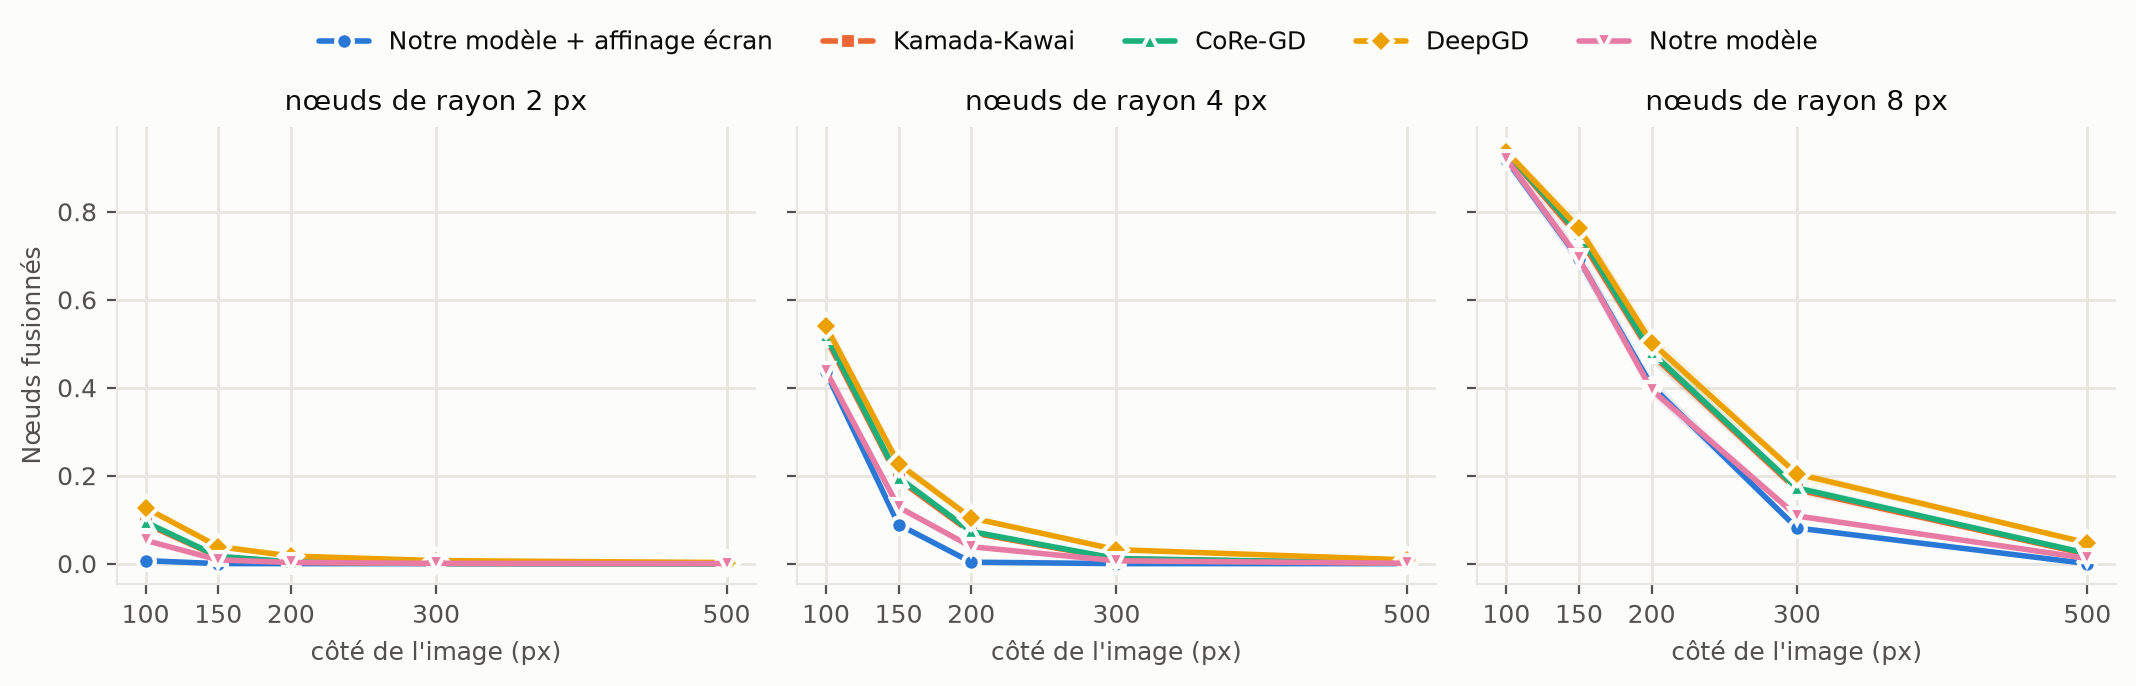
\includegraphics[width=0.92\textwidth]{yani_fusionnes.png}

\vspace{0.05cm}
\begin{minipage}{0.97\textwidth}
\footnotesize
\begin{itemize}
\setlength{\itemsep}{2pt}
\item Nœuds de 4 px, Kamada-Kawai : \textbf{0 \% de nœuds fusionnés à 500 px, 7 \% à 200 px, 19 \% à 150 px, 51 \% à 100 px}. CoRe-GD et DeepGD de même.
\item \textbf{Affiné à l'écran au réglage cible} : 0,3 \% à 200 px, 9 \% à 150 px ; stress inchangé (0,061).
\item Notre affinage réglé pour 500 px fait \emph{pire} que le modèle seul à 150 px (17 \% contre 13 \%) : dessiner pour le mauvais écran coûte.
\end{itemize}
\end{minipage}
\end{frame}

\begin{frame}{Résultat 2 : écran contre témoin géométrique}
\centering
\footnotesize
\setlength{\tabcolsep}{4pt}
\resizebox{\textwidth}{!}{%
\begin{tabular}{@{}l ccc ccc@{}}
\toprule
 & \multicolumn{3}{c}{\textbf{Nœuds fusionnés} $\downarrow$} & \multicolumn{3}{c}{\textbf{Arêtes ambiguës / arête} $\downarrow$} \\
\cmidrule(lr){2-4}\cmidrule(lr){5-7}
\textbf{Départ KK} & 150 px, 2 px & 200 px, 4 px & 300 px, 4 px & 150 px, 2 px & 200 px, 4 px & 300 px, 4 px \\
\midrule
sans affinage & 1,6 \% & 7,0 \% & 1,1 \% & 0,130 & 0,187 & 0,108 \\
témoin géométrique & 1,6 \% & 7,1 \% & 0,4 \% & 0,129 & 0,174 & 0,118 \\
témoin, marge de 2 px & 0 \% & 0,7 \% & 0 \% & 0,056 & 0,127 & 0,034 \\
\textcolor{bleu}{\textbf{écran}} & \textbf{0 \%} & \textbf{0,9 \%} & \textbf{0 \%} & \textbf{0,042} & \textbf{0,100} & \textbf{0,020} \\
\bottomrule
\end{tabular}}

\vspace{0.35cm}
\begin{minipage}{0.95\textwidth}
\footnotesize
\begin{itemize}
\setlength{\itemsep}{2pt}
\item À budget et sélection égaux, \textbf{l'écran bat le témoin sans marge} sur les fusions (26 réglages sur 32) et les arêtes ambiguës (32 sur 32). Wilcoxon apparié, Holm sur 384 tests.
\item \textbf{Mais une marge de 2 px suffit au témoin pour les nœuds} (il fait même mieux dans 12 cas sur 32) : pour des disques, le gain vient de l'échelle du pixel, qu'une loss géométrique peut recevoir.
\item \textbf{Pour les arêtes qui touchent un nœud, l'écran reste meilleur} même contre la marge (29 sur 32, jamais moins bon), avec moins de croisements. Stress identique partout.
\end{itemize}
\end{minipage}
\end{frame}

\begin{frame}{Des arêtes courbes, optimisées à l'écran}
\begin{columns}[c]
\begin{column}{0.48\textwidth}
\centering
{\scriptsize arêtes droites \hspace{2.2cm} arêtes courbes}\\[2pt]
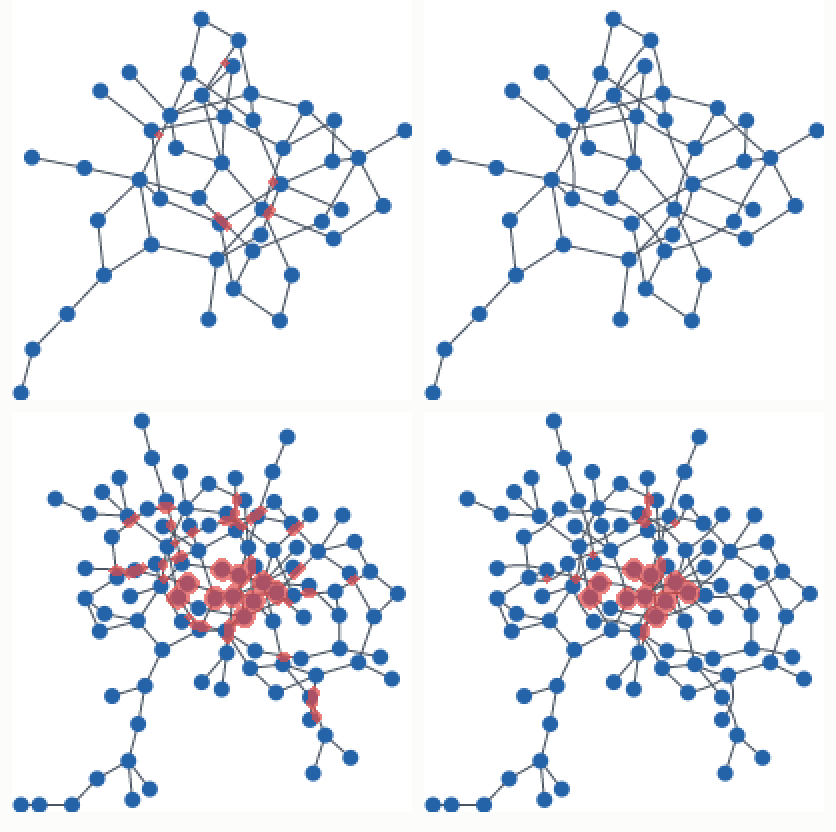
\includegraphics[height=0.72\textheight]{yani_courbes.png}
\end{column}
\begin{column}{0.5\textwidth}
\small
\begin{itemize}
\setlength{\itemsep}{4pt}
\item Une Bézier quadratique par arête ; on optimise son point de contrôle, \textbf{les nœuds ne bougent pas}.
\item SDF exacte du trait (polyligne à jointures rondes) ; pertes : courbe sur un nœud, courbe sur une courbe, croisements, courbure.
\item Après l'affinage écran, \textbf{arêtes ambiguës $-74$\,\%} à 200 px (0,091 $\to$ 0,024), $-34$ à $-42$\,\% sur les deux autres réglages, un peu moins de croisements.
\item Contrepartie : arêtes confondues $+0{,}5$ à $+0{,}9$ point.
\end{itemize}
\end{column}
\end{columns}
\end{frame}

\begin{frame}{Impact environnemental : mesures}
\centering
\footnotesize
\renewcommand{\arraystretch}{0.9}
\begin{tabular}{@{}lccc@{}}
\toprule
\textbf{Calcul} (deepeirb, un GPU RTX 6000 Ada) & \textbf{Durée} & \textbf{Énergie} & \textbf{CO$_2$eq} \\
\midrule
Entraînement (phases 1 et 2) & 28 min & 0,049 à 0,062 kWh & 3,5 g \\
Benchmark, balayage, témoins, courbes & 1 h 30 & 0,26 à 0,28 kWh & 16 g \\
\midrule
\textbf{Total mesuré} & \textbf{1 h 57} & \textbf{0,31 à 0,35 kWh} & \textbf{19 g} \\
\bottomrule
\end{tabular}

\vspace{0.12cm}
\begin{tabular}{@{}lcc@{}}
\toprule
\textbf{Par dessin} (graphe de Rome) & \textbf{Temps} & \textbf{Énergie} \\
\midrule
Kamada-Kawai (CPU) & 24 ms & 0,55 mWh \\
Notre modèle (GPU) & 14 ms & 0,38 mWh \\
Affinage écran, par paquets (GPU) & 10 à 14 ms & 0,29 à 0,51 mWh \\
\bottomrule
\end{tabular}

\vspace{0.08cm}
\begin{minipage}{0.95\textwidth}
\scriptsize
\begin{itemize}
\setlength{\itemsep}{1pt}
\item \texttt{codecarbon} hors ligne, réseau français (56 g/kWh), scripts lancés sous \texttt{run\_tracked.py}. Fourchettes : codecarbon comptait aussi le GPU inutilisé (19 à 27 W au repos), corrigé depuis.
\item \textbf{Entraînement remboursé après environ 300\,000 dessins} face à Kamada-Kawai : sur des graphes de Rome, KK est déjà bon marché.
\item L'affinage coûte selon le nombre de défauts, pas la taille de l'image (plus cher à 100 px qu'à 500 px).
\end{itemize}
\end{minipage}
\end{frame}

\end{document}
